\chapter{Acquisition-System Design}
\section{Overview}
This section covers the complete development process including the hardware, gateware, software and mechanical design of the project.
It is important to note that the following documentation concentrates only on the final version of the device. Earlier hardware prototypes are not covered due to the lack of relevance.

\subsection{Key Requirements}
The main focus of the development is to design a professional looking, easy to use and eye-catching device for demonstration purposes.
The project name \textit{Audio-Beamformer} has been chosen as it is easy to remember and has potential to be seen as a trademark.

The following key requirements have been set:
\begin{itemize}
	\item Single power adapter or power cable (e.g. no need of labor power supplies)
	\item Easy to install (e.g. montage on a camera tripod)
	\item Intuitive to operate via state-of-the-art graphical user interface
	\item Multiple audio streaming sources such as Bluetooth and USB input devices
	\item Great scalability and flexibility of the hardware and software design
\end{itemize}

\subsection{Key Decisions}
In the conceptional phase of the development, several key decisions had to be made.
This contains mainly the signal flow and the division between the processing part on the Raspberry Pi and the \acrshort{fpga}.
Further, the question had to be evaluated, if a built-in power supply or an external power adapter is preferred.
And most importantly, which type of ultrasonic transducer should be used in the design.
In addition, the overall dimension and scale of the final product had to be discussed.
In general, most of these decisions were made according to results of simulations, physical measurements and after extensive discussions.
In the following sections, each part of the project is explained in detail.


\newpage
\section{Hardware Design}

\begin{figure}[h]
	\centering
	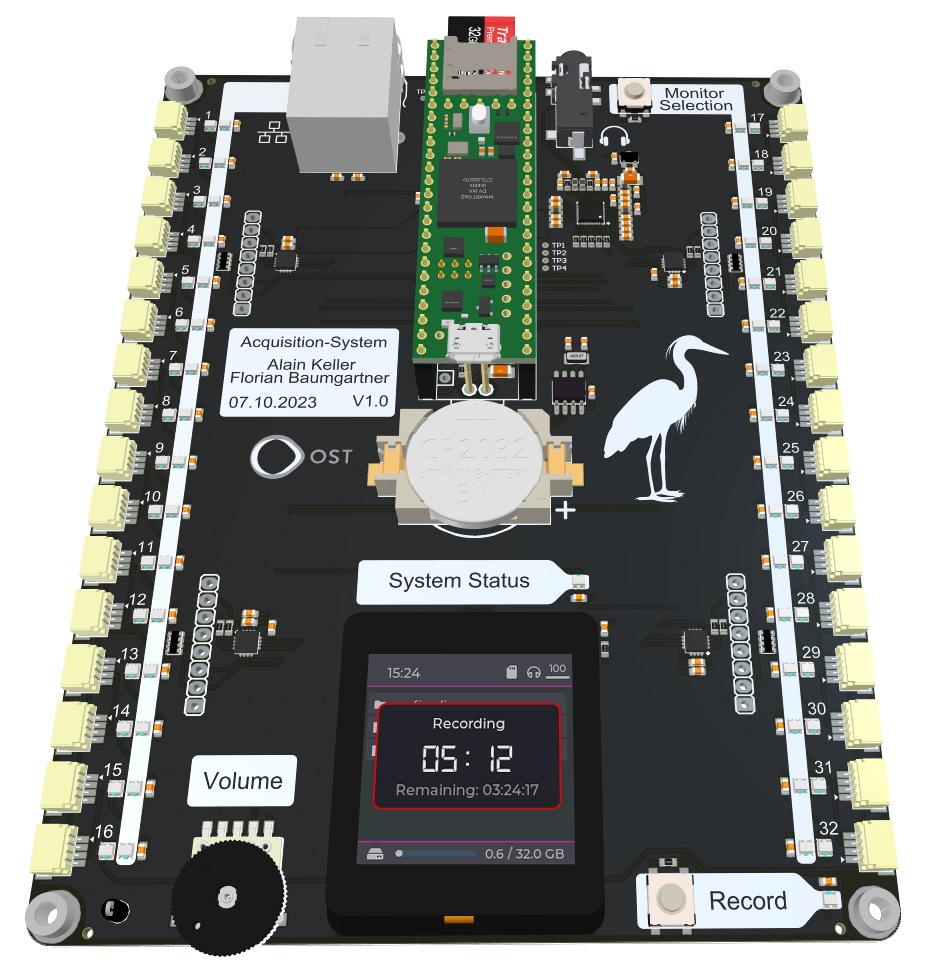
\includegraphics[width=1.0\textwidth]{images/4_design_acquisition_system/Acquisition_System_Front.png}
	\caption{Front view of the Acquisition System}
	\label{fig:acquisition_system_front}
\end{figure}


\subsection{Block Diagram}

\begin{figure}[h]
	\centering
	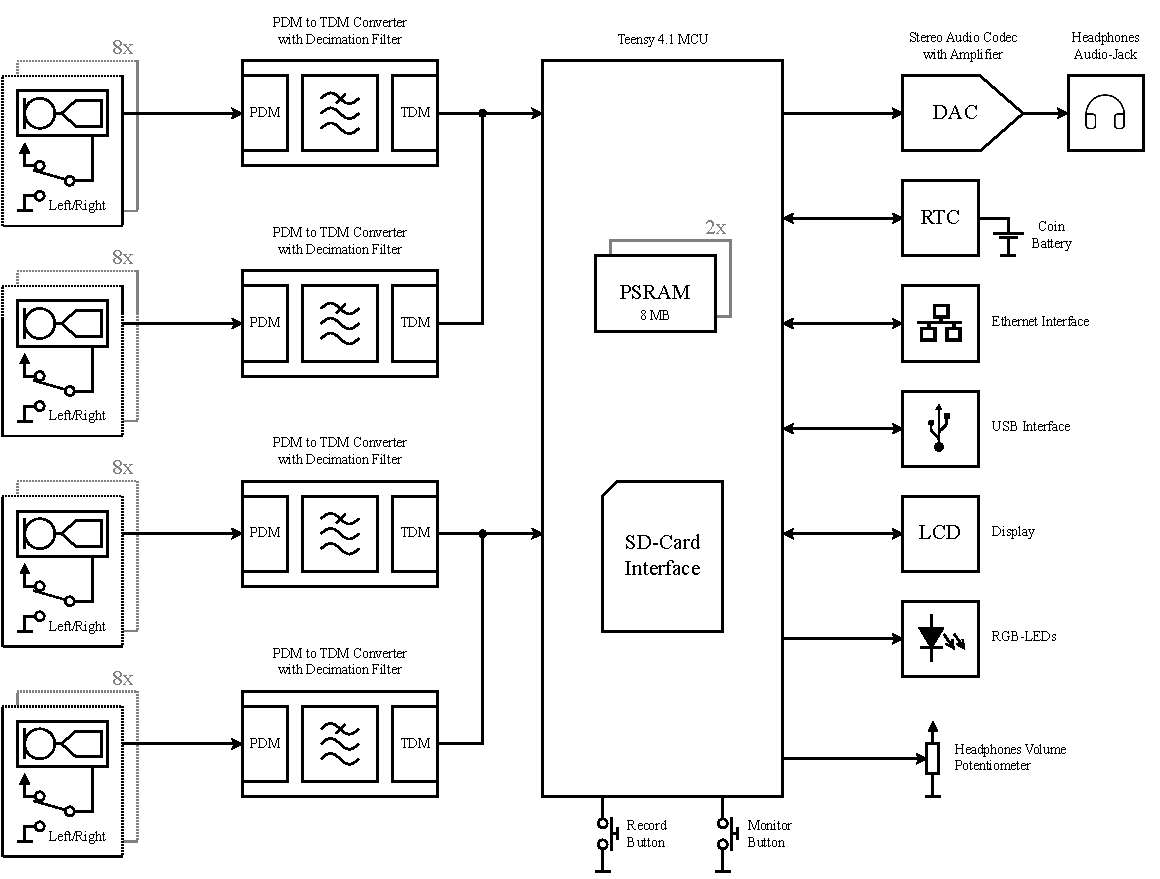
\includegraphics[width=1.0\textwidth]{images/4_design_acquisition_system/system_block_diagram.pdf}
	\caption{System block diagram}
	\label{fig:system_block_diagram}
\end{figure}

\subsection{Microcontroller Unit (MCU)}

%  TODO: Write about external PSRAM


\subsection{Audio Input}

\subsection{Audio Processing}

\subsection{Headphone Output}

To prelisten the individual audio channels, a headphone output is implemented.

% description of headphones jack
The headphone output is a standard 3.5mm stereo jack.



\newpage
\section{Firmware Design}
Blabla



